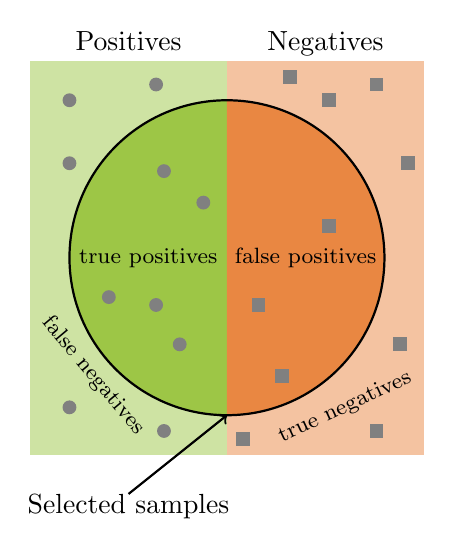
\begin{tikzpicture}
  \tikzset{every node/.style={inner sep=0,outer sep=0}}

  \definecolor{positive}{RGB}{132, 184, 24}
  \definecolor{negative}{RGB}{227, 105, 19}

  \node[above] at (1.25, 5) {\strut Positives};
  \begin{scope}
    \clip (0, 0) rectangle (2.5, 5);
    \fill[positive!40] (0, 0) rectangle (2.5, 5);
    \fill[positive!80] (2.5, 2.5) circle [radius=2];
  \end{scope}


  \node[above] at (3.75, 5) {\strut Negatives};
  \begin{scope}
    \clip (5, 0) rectangle (2.5, 5);
    \fill[negative!40] (5, 0) rectangle (2.5, 5);
    \fill[negative!80] (2.5, 2.5) circle [radius=2];
  \end{scope}

  \draw[thick] (2.5, 2.5) circle [radius=2];

  \foreach \xy in {
    (0.5, 0.6), (0.5, 4.5), (1.7, 3.6), (1., 2.0), (0.5, 3.7),
    (1.6, 4.7), (1.9, 1.4), (2.2, 3.2), (1.6, 1.9), (1.7, 0.3)
  } {
    \node[fill=gray, circle, minimum size=5pt] at \xy {};
  }
  \foreach \xy in {
    (3.8, 2.9), (4.4, 0.3), (3.8, 4.5), (4.4, 4.7), (4.7, 1.4),
    (2.9, 1.9), (3.3, 4.8), (3.2, 1.0), (4.8, 3.7), (2.7, 0.2)
  } {
    \node[fill=gray, rectangle, minimum size=5pt] at \xy {};
  }
  \draw[thick, <-] (2.5, 0.5) -- (1.25, -0.5) node[below]{Selected samples};
  \node[] at (1.5, 2.5) {\footnotesize true positives};
  \node[] at (3.5, 2.5) {\footnotesize false positives};
  \node[rotate=25] at (4, 0.6) {\footnotesize true negatives};
  \node[rotate=-50] at (0.8, 1.0) {\footnotesize false negatives};
\end{tikzpicture}
